\PassOptionsToPackage{unicode=true}{hyperref} % options for packages loaded elsewhere
\PassOptionsToPackage{hyphens}{url}
%
\documentclass[ignorenonframetext,]{beamer}
\usepackage{pgfpages}
\setbeamertemplate{caption}[numbered]
\setbeamertemplate{caption label separator}{: }
\setbeamercolor{caption name}{fg=normal text.fg}
\beamertemplatenavigationsymbolsempty
% Prevent slide breaks in the middle of a paragraph:
\widowpenalties 1 10000
\raggedbottom
\setbeamertemplate{part page}{
\centering
\begin{beamercolorbox}[sep=16pt,center]{part title}
  \usebeamerfont{part title}\insertpart\par
\end{beamercolorbox}
}
\setbeamertemplate{section page}{
\centering
\begin{beamercolorbox}[sep=12pt,center]{part title}
  \usebeamerfont{section title}\insertsection\par
\end{beamercolorbox}
}
\setbeamertemplate{subsection page}{
\centering
\begin{beamercolorbox}[sep=8pt,center]{part title}
  \usebeamerfont{subsection title}\insertsubsection\par
\end{beamercolorbox}
}
\AtBeginPart{
  \frame{\partpage}
}
\AtBeginSection{
  \ifbibliography
  \else
    \frame{\sectionpage}
  \fi
}
\AtBeginSubsection{
  \frame{\subsectionpage}
}
\usepackage{lmodern}
\usepackage{amssymb,amsmath}
\usepackage{ifxetex,ifluatex}
\usepackage{fixltx2e} % provides \textsubscript
\ifnum 0\ifxetex 1\fi\ifluatex 1\fi=0 % if pdftex
  \usepackage[T1]{fontenc}
  \usepackage[utf8]{inputenc}
  \usepackage{textcomp} % provides euro and other symbols
\else % if luatex or xelatex
  \usepackage{unicode-math}
  \defaultfontfeatures{Ligatures=TeX,Scale=MatchLowercase}
\fi
% use upquote if available, for straight quotes in verbatim environments
\IfFileExists{upquote.sty}{\usepackage{upquote}}{}
% use microtype if available
\IfFileExists{microtype.sty}{%
\usepackage[]{microtype}
\UseMicrotypeSet[protrusion]{basicmath} % disable protrusion for tt fonts
}{}
\IfFileExists{parskip.sty}{%
\usepackage{parskip}
}{% else
\setlength{\parindent}{0pt}
\setlength{\parskip}{6pt plus 2pt minus 1pt}
}
\usepackage{hyperref}
\hypersetup{
            pdftitle={Introduction to Deep learning with R for dummies by dummies},
            pdfauthor={S. Donnet},
            pdfborder={0 0 0},
            breaklinks=true}
\urlstyle{same}  % don't use monospace font for urls
\newif\ifbibliography
\usepackage{graphicx,grffile}
\makeatletter
\def\maxwidth{\ifdim\Gin@nat@width>\linewidth\linewidth\else\Gin@nat@width\fi}
\def\maxheight{\ifdim\Gin@nat@height>\textheight\textheight\else\Gin@nat@height\fi}
\makeatother
% Scale images if necessary, so that they will not overflow the page
% margins by default, and it is still possible to overwrite the defaults
% using explicit options in \includegraphics[width, height, ...]{}
\setkeys{Gin}{width=\maxwidth,height=\maxheight,keepaspectratio}
\setlength{\emergencystretch}{3em}  % prevent overfull lines
\providecommand{\tightlist}{%
  \setlength{\itemsep}{0pt}\setlength{\parskip}{0pt}}
\setcounter{secnumdepth}{0}

% set default figure placement to htbp
\makeatletter
\def\fps@figure{htbp}
\makeatother


\title{Introduction to Deep learning with R for dummies by dummies}
\author{S. Donnet}
\date{Paris, March 2019}

\begin{document}
\frame{\titlepage}

\hypertarget{introduction-supervised-learning}{%
\section{Introduction : supervised
learning}\label{introduction-supervised-learning}}

\begin{frame}{Example: Digit Recognition}
\protect\hypertarget{example-digit-recognition}{}

\begin{figure}
\centering
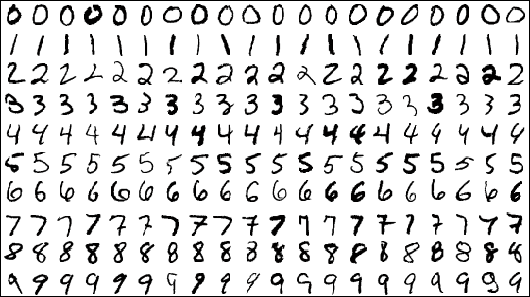
\includegraphics{mnist.png}
\caption{Recognition of handwritten digits}
\end{figure}

\end{frame}

\begin{frame}{Example: Digit Recognition}
\protect\hypertarget{example-digit-recognition-1}{}

\begin{figure}
\centering
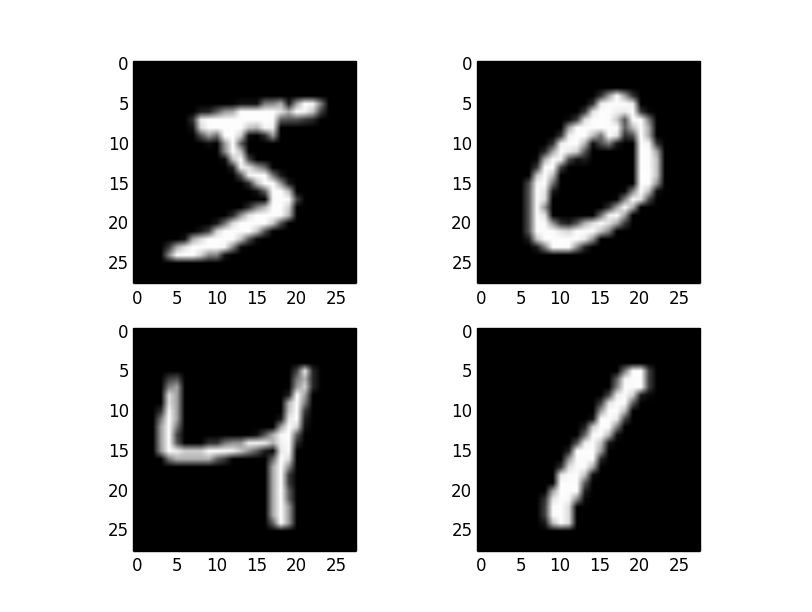
\includegraphics[width=2.60417in,height=\textheight]{mnist_details.png}
\caption{Recognition of handwritten digits}
\end{figure}

\begin{itemize}
\tightlist
\item
  Each image \(i\) of digit is of size \(28 \times 28 = 784\) pixels
\item
  Each pixel \(j\) is associated with a gray level
  \(x_i^j \in \{0, \dots, 255 \}\)
\end{itemize}

\end{frame}

\begin{frame}{Example: Digit Recognition}
\protect\hypertarget{example-digit-recognition-2}{}

\begin{itemize}
\item
  The gray levels are stored in a vector
  \(\mathbf{x}_i = (x_i^r)_{r = 1 \dots p}\), \(p = 784\)
\item
  \(y_i \in \{0, \dots, 9\}\): image label

  \begin{itemize}
  \tightlist
  \item
    \(y_i\) : observed / known for a learning sample
  \item
    \(y\) must be predicted for a new image \(\mathbf{x}\)
  \end{itemize}
\end{itemize}

\end{frame}

\begin{frame}{Formally}
\protect\hypertarget{formally}{}

\begin{itemize}
\item
  We consider \(n\) objects (images, texts, sound \ldots{}), described
  by \(p\) characteristics.
\item
  For each object \(i\), these characteristics are stored in a vector
  \(\mathbf{x}_i = (x_i^1, \dots, x_i^p)\) of \(\mathbb{R}^p\).
\item
  An output variable \(y_i\) is each object \(i\) is assigned

  \begin{itemize}
  \tightlist
  \item
    If \(y_i \in \mathbb{R}^d\): we talk about regression
  \item
    If \(y_i \in E\) with \(E\) set, we talk about - discriminating if
    \(E = \{0,1 \}\); - classification if \(E = \{0, \dots, 9\}\) for
    example - shape recognition if
    \(E = \{\text {dog}, \text {groundhog}, ... \}\)
  \end{itemize}
\item
  \textbf {Goal}: predict the output \(y\) for a new set of
  characteristics \(\mathbf{x}\)
\item
  \textbf{How do we do it?}: learn (on a set of learning data =
  training) a prediction rule or classification and provide this rule to
  apply it to \(\mathbf{x}\)
\end{itemize}

\end{frame}

\begin{frame}{Other examples}
\protect\hypertarget{other-examples}{}

\begin{itemize}
\tightlist
\item
  Face recognition on pictures \(E = \{\) family members \(\}\)
\item
  Recognition of the political edge by speach analysis
\end{itemize}

\end{frame}

\begin{frame}{What's the difference between estimation and learning?}
\protect\hypertarget{whats-the-difference-between-estimation-and-learning}{}

\begin{itemize}
\item
  Statistical tradition / estimation :

  \begin{itemize}
  \tightlist
  \item
    Concept of model is central with an explanatory purpose
  \item
    Seeking to approach reality, propose a model possibly based on a
    physical theory, economic,
  \item
    Interpretation of the role of each explanatory variable in the
    process is important.
  \end{itemize}
\item
  Learning: the objective is essentially the prediction,

  \begin{itemize}
  \tightlist
  \item
    best model is not necessarily the one that best fits the true model.
  \item
    theoretical framework is different and error control requires
    another approach: choices based on prediction quality criteria
  \item
    Interpretability is less important
  \end{itemize}
\end{itemize}

\end{frame}

\begin{frame}{So what about the good old (generalized) linear model?}
\protect\hypertarget{so-what-about-the-good-old-generalized-linear-model}{}

\[ y_i \sim  \mathcal{F} \quad \mbox{ with } \quad \phi(\mathbb{E}[y_i]) = \mathbf{x}^T\beta\]

\begin{itemize}
\tightlist
\item
  If the dimensions of the problem \((n, p)\) are reasonable
\item
  If model assumptions (linearity) and distributions are verified
\item
  THEN: statistical modeling techniques issued from the general linear
  model are optimal (maximum likelihood)
\item
  We will not do better, especially in the case of small samples
\end{itemize}

\end{frame}

\begin{frame}{But\ldots{}}
\protect\hypertarget{but}{}

\begin{itemize}
\tightlist
\item
  As soon as the distribution hypotheses are not verified,
\item
  As soon as the supposed relations between the variables or with the
  variable of interest are not linear
\item
  As soon as the data volume is important (big data),
\end{itemize}

We will consider other methods that will over-rate rudimentary
statistical models.

\end{frame}

\hypertarget{deep-learning}{%
\section{Deep learning}\label{deep-learning}}

\begin{frame}{Deep learning: introduction}
\protect\hypertarget{deep-learning-introduction}{}

\begin{itemize}
\tightlist
\item
  Definition (attempt): set of learning methods that attempt to model
  data with complex architectures combining various non-linear
  transformations
\end{itemize}

\[ \mathbf{x} \mapsto f(\mathbf{x},\theta) \mbox{ such that } y \simeq f(\mathbf{x},\theta)\]

\begin{itemize}
\tightlist
\item
  The basic building blocks of Deep Learning are \textbf{neural
  networks}.
\item
  These bricks are combined to form \textbf{deep neural networks}.
\end{itemize}

\end{frame}

\begin{frame}{Application areas}
\protect\hypertarget{application-areas}{}

These techniques have led to significant progress in the following
areas:

\begin{itemize}
\tightlist
\item
  image and sound processing: facial recognition, automatic speech
  recognition (transformation of a voice into written text),
\item
  computer vision: to imitate the human vision (machine seeing several
  objects at once),
\item
  automatic processing of natural language,
\item
  text classification (eg spam detection).
\end{itemize}

Infinite amount of potential applications

\end{frame}

\begin{frame}{Different types of architectures for neural networks}
\protect\hypertarget{different-types-of-architectures-for-neural-networks}{}

\begin{itemize}
\item
  \emph{Multilayer Perceptrons}: the oldest and simplest
\item
  \emph{Convolutional neural networks}: very efficient for image
  processing
\item
  \emph{Recurrent neural networks}, useful for sequential data (texts or
  time series)
\item
  All are based on deep layers of layers
\item
  Requires intelligent optimization algorithms (stochastic in general),
  careful initialization and a smart choice of structure.
\item
  Impressive results but few theoretical justifications for the moment
\end{itemize}

\end{frame}

\begin{frame}{Artificial neuron}
\protect\hypertarget{artificial-neuron}{}

\begin{itemize}
\item
  \emph{A neuron} is a non-linear application in its parameters that
  associates an output \(f(\mathbf{x})\) to an input vector
  \(\mathbf{x}\):
\item
  More precisely, the \(j\)-th neuron \(f_j\) is written\\
  \[f_j (\mathbf{x}) = \phi (<w_j, \mathbf {x}> + b_j)\] where

  \begin{itemize}
  \tightlist
  \item
    \(<w_j, \mathbf{x}> = \sum_{r = 1}^p w_j^r x^r\)
  \item
    The quantities \(w_j = (w_j^1, \dots, w_j^p)\) are the weights of
    the input variables \((x^1, \dots, x^p)\)
  \item
    \(b_j\)is the bias of neuron \(j\).
  \item
    \(\phi\) is the activation function
  \end{itemize}
\end{itemize}

\end{frame}

\begin{frame}{Basic model involving one neuron}
\protect\hypertarget{basic-model-involving-one-neuron}{}

We explain the output variable \(y\) by
\[ y \simeq f(\mathbf{x},\theta) =  \phi(<w,\mathbf{x}> + b)\]

\begin{itemize}
\tightlist
\item
  If \(\phi(z) =z\) and we only have one neurone \(\Rightarrow\)
  classical linear function
\end{itemize}

\end{frame}

\begin{frame}{Choice of the activation function \(\phi\)}
\protect\hypertarget{choice-of-the-activation-function-phi}{}

\begin{itemize}
\item
  If \(Y \in \{0,1\}\) and we want to predict \(P(Y=1|x)\) : logistic
  function \[\phi(z) = \frac{1}{1+e^{-z}} \in [0,1]\]
\item
  \emph{Generalization}: If \(Y \in E\) (\(E\) finite space of cardinal
  \(K\)) and we want to predict \(P(Y= e|x)\) : \(softmax\)
  \[\phi(z_1, \dots, z_K) =\left(\frac{e^{z_j}}{\sum_{j = 1\dots K} e^{z_j}}\right)_{j=1\dots K}\]
\item
  Hyperbolic tangent function :
  \(\phi = \tanh:\mathbb{R} \mapsto [-1,1]\)
\item
  Threshold function : \(\phi(z) = 1_{z>s} \in \{0,1\}\)
\item
  Rectified linear unit (ReLU) \(\phi(z) = max(z,0)\)

  \begin{itemize}
  \tightlist
  \item
    OK to predict positive values. Continuous but non differentiable
  \end{itemize}
\end{itemize}

\end{frame}

\begin{frame}{Plots}
\protect\hypertarget{plots}{}

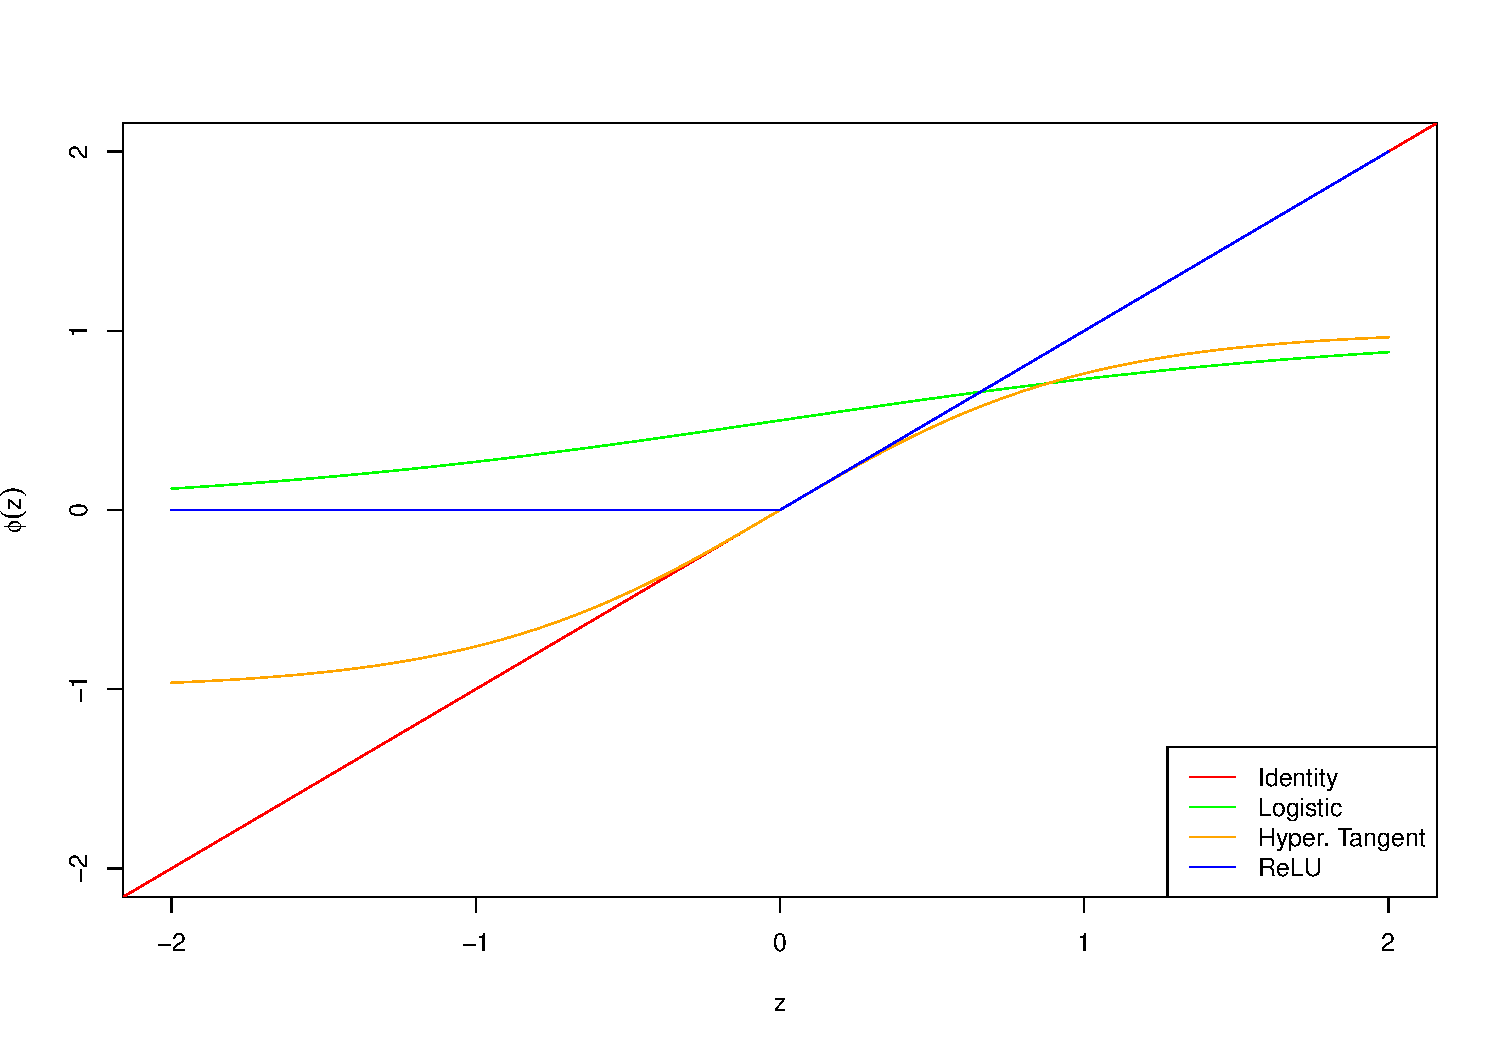
\includegraphics{cours_deeplearning_for_dummies_files/figure-beamer/unnamed-chunk-1-1.pdf}

Various differentiability properties : important when we will have to
optimize the \(w\) et \(b\)

\end{frame}

\begin{frame}{Neural networks or multilayer perceptrons}
\protect\hypertarget{neural-networks-or-multilayer-perceptrons}{}

\begin{itemize}
\tightlist
\item
  Structure composed of different hidden layers of neurons whose outputs
  serve as inputs to the neurons of the next layer
\item
  Activation functions are the same in the different layers, only the
  last is different (adapted to the objective: classification or
  regression)
\end{itemize}

\end{frame}

\begin{frame}{Example}
\protect\hypertarget{example}{}

\begin{figure}
\centering
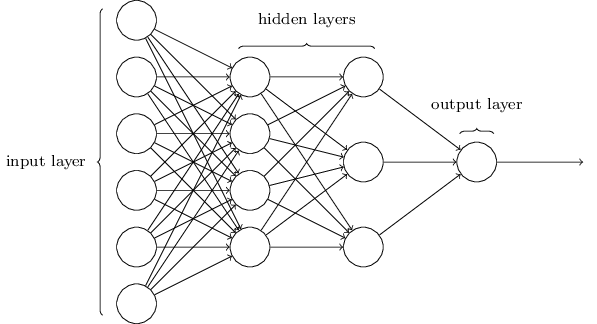
\includegraphics[width=2.60417in,height=\textheight]{mlp-network.png}
\caption{Example of neural network}
\end{figure}

\begin{itemize}
\tightlist
\item
  Input layer : as many nodes as variables \(x\) : \(p\)\\
\item
  Hidden layer : number of neurons, to be set but the user (here 4 then
  3)
\item
  Output layer : 1 node = \(y\) for regression or binary classif and
  number of modalities for general classification
\end{itemize}

\end{frame}

\begin{frame}[fragile]{Neural network : formally}
\protect\hypertarget{neural-network-formally}{}

Let \(J_{\ell}\) be the number of neurons in layer \(\ell\)

\begin{itemize}
\item
  Layer \(0\) : \(h^0(\mathbf{x}) = \mathbf{x} \in \mathbb{R}^p\)
\item
  For hidden layers \(\ell = 1\dots L\):

  \begin{itemize}
  \tightlist
  \item
    We create \(J_{\ell}\) neurons : for every \(j = 1 \dots J_{\ell}\)
    :
  \end{itemize}

  \begin{eqnarray*}
        a^{(\ell)}_j(\mathbf{x}) &=& b^{(\ell)}_j + \sum_{m=1}^{J_{\ell-1}} W^{(\ell)}_{jm} h_m^{(\ell-1)}(\mathbf{x}) \\
        &=& b^{(\ell)}_j + < W^{(\ell)}_{j},  h ^{(\ell-1)}(\mathbf{x}) >
        \end{eqnarray*}

\begin{verbatim}
  $$h_j^{(\ell)}(\mathbf{x}) = \phi(a_j^{(\ell)}(\mathbf{x}))$$
\end{verbatim}
\item
  With vectors and matrices :
  \[a^{(\ell)}(\mathbf{x}) = b^{(\ell)} +W^{(\ell)} h^{(\ell-1)}(\mathbf{x}) \in \mathbb{R}^{J_{\ell}}\]
  \[h^{(\ell)}(\mathbf{x}) = \phi(a^{(\ell)}(\mathbf{x}))\] where
  \(W^{(\ell)}\) is matrix of size \(J_{\ell} \times J_{\ell-1}\)
\end{itemize}

\end{frame}

\begin{frame}{Neural network: formally}
\protect\hypertarget{neural-network-formally-1}{}

\begin{itemize}
\tightlist
\item
  For the last layer \(\ell = L+1\):
\end{itemize}

\[a^{(L+1)}(\mathbf{x}) = b^{(L+1)} +W^{(L+1)} h^{(L)}(\mathbf{x}) \in \mathbb{R}^J\]
\[h^{(L+1)}(\mathbf{x}) = \psi(a^{(L+1)}(\mathbf{x}))\]

\end{frame}

\begin{frame}{Neural network: finally}
\protect\hypertarget{neural-network-finally}{}

\begin{itemize}
\tightlist
\item
  \(W^{(\ell)}\) is a weight matrix with \(J_{\ell}\) rows and
  \(J_{\ell-1}\) columns.\\
\item
  \(W^{(L+1)}\) is a weight matrix with \(1\) row and \(J_{L}\) colums
  \(y \in \mathbb{R}\)
\item
  \[\mathbf{x} \mapsto f(\mathbf{x},\theta) = \psi(a^{(L+1)}(\mathbf{x}))\]
  - If we are in a regression context \(\psi(z) = z\),\\
  - If we are in a binary classification context \(\psi\) is the sigmoid
  function (prediction in \([0,1]\)).\\
  - If we are in a multiclass classification framework :
  \(\psi = softmax\)
\end{itemize}

\end{frame}

\begin{frame}{Neural Network:}
\protect\hypertarget{neural-network}{}

\begin{itemize}
\item
  Basic architecture since each layer depends on the previous layer and
  not on the neurons of the same layer (\(\Rightarrow\) recurrent neural
  networks)
\item
  Parameters to tune or fit: - number of layers - number of neurons in
  each layer - hidden layer activation functions (\(\phi\)) - Choice of
  the output activation function (\(\psi\)) driven by the dataset
\end{itemize}

\end{frame}

\begin{frame}{Recurrent neural networks}
\protect\hypertarget{recurrent-neural-networks}{}

\begin{itemize}
\tightlist
\item
  The output of a neuron can be the input of a neuron of the same layer.
\end{itemize}

\end{frame}

\begin{frame}{Theoretical result}
\protect\hypertarget{theoretical-result}{}

\begin{itemize}
\item
  Hornik (1991) proved that any smooth bounded function from
  \(\mathbb{R}^p\) to \(\mathbb{R}\) can be approximated by a one layer
  neural network with a finite number of neurons with the same
  activation function \(\phi\) and \(\psi = id\).
\item
  Interesting result from a theoretical point of view.
\item
  In practice :

  \begin{itemize}
  \tightlist
  \item
    Required number of neurons can be very large.
  \item
    Strength of deep leargning derives from the number of hidden layers
  \end{itemize}
\end{itemize}

\end{frame}

\hypertarget{parameters-estimation}{%
\section{Parameters estimation}\label{parameters-estimation}}

\begin{frame}{A quantity to minimize / maximize : loss function}
\protect\hypertarget{a-quantity-to-minimize-maximize-loss-function}{}

\begin{itemize}
\tightlist
\item
  Parameters to estimate : \(\theta\) = weights \(W^{(\ell)}\) ans bias
  \(b^{(\ell)}_j\)
\item
  Classically : estimation by maximizing the (\(\log\))-likelihood\\
\item
  Loss function: \(=-\log\;\) likelihood

  \begin{itemize}
  \item
    In the regression framework :
    \(Y \sim \mathcal{N}(f(\mathbf{x},\theta), I)\)
    \[ \ell(f(\mathbf{x},\theta),Y) = \| Y - f(\mathbf{x},\theta)\|^2\]
  \item
    For the binary classification \(\{0,1\}\) :
    \(Y \sim \mathcal{B}(1,f(\mathbf{x},\theta))\)
    \[ \ell(f(\mathbf{x},\theta),Y) = -Y \log(f(\mathbf{x},\theta)) - (1-Y) \log(1- f(\mathbf{x},\theta))\]
    (cross-entropy)
  \item
    For the multiclass classification
    \[ \ell(f(\mathbf{x},\theta),Y) =-\sum_{e \in E} \mathbf{1}_{Y=e} \log p_{\theta}(Y = e | \mathbf{x} )\]
  \end{itemize}
\end{itemize}

\end{frame}

\begin{frame}{Loss function: remark}
\protect\hypertarget{loss-function-remark}{}

\begin{itemize}
\tightlist
\item
  Ideally, we would like to minimize the classification error but it is
  not a differentiable function
\item
  So we resort to the ``cross-entropy'' which can be differentiated
\end{itemize}

\end{frame}

\begin{frame}{Penalized empirical risk}
\protect\hypertarget{penalized-empirical-risk}{}

Risk \[\mathbb{E}_{Y}[\ell(f(\mathbf{x},\theta),Y)]\] replaced by the
empirical risk \(\mathbb{E}_{Y}[\ell(f(\mathbf{x},\theta),Y)]\)

\begin{itemize}
\tightlist
\item
  For a training sample \((\mathbf{x}_i,Y_i)_{i=1\dots n}\)
\end{itemize}

\[ L_n(\theta) = \frac{1}{n}\sum_{i=1}^n  \ell(f(\mathbf{x}_i,\theta),Y_i)\]

\begin{itemize}
\tightlist
\item
  Penalization :
  \[ L_n(\theta) = \frac{1}{n}\sum_{i=1}^n  \ell(f(\mathbf{x}_i,\theta),Y_i) + \lambda \Omega(\theta) \]
  with, for instance,
  \(\Omega(\theta) = \sum_{\ell,i,j} (W^{(\ell)}_{ij})^2\) or
  \(\Omega(\theta) = \sum_{\ell,i,j} |W^{(\ell)}_{ij}|\) to avoid
  overfitting.
\end{itemize}

\end{frame}

\begin{frame}{Minimization by Stochastic gradient descent.}
\protect\hypertarget{minimization-by-stochastic-gradient-descent.}{}

\textbf{Algorithm (by Rumelhart et al (1988))}

\begin{itemize}
\item
  Choose an initial value of parameters \(\theta\) and a learning rate
  \(\eta\)
\item
  Repeat until a minimum is reached:

  \begin{itemize}
  \tightlist
  \item
    Split randomy the training set into \(N_B\) \emph{batches} of size
    \(m\) (\(n = m \times N_B\))
  \item
    for each batch \(B\) set:
    \[ \theta:= \theta - \eta \frac{1}{m}\sum_{i \in B} \nabla_{\theta} \left\{  \ell(f(\mathbf{x}_i,\theta),Y_i) + \lambda   \Omega(\theta)\right\}\]
  \end{itemize}
\end{itemize}

\textbf{Remarks}:

\begin{itemize}
\item
  Each iteration is called an \emph{epoch}.
\item
  The number of epochs is a parameter to tune
\item
  Difficulty comes from the computation of the gradient
\end{itemize}

\end{frame}

\begin{frame}{Calculus of the gradient for the regression}
\protect\hypertarget{calculus-of-the-gradient-for-the-regression}{}

\begin{itemize}
\tightlist
\item
  \(Y \in \mathbb{R}\).
\item
  \(R_i = \ell(f(\mathbf{x}_i,\theta),Y_i) = (Y_{i} - f(\mathbf{x}_i,\theta))^2\)
\item
  For any activation function \(\phi\) (hidden layers) and \(\psi\)
\end{itemize}

\end{frame}

\begin{frame}{Partial derivatives of \(R_i\) with respect to the weights
of the last layer}
\protect\hypertarget{partial-derivatives-of-r_i-with-respect-to-the-weights-of-the-last-layer}{}

\begin{itemize}
\item
  Derivatives of
  \(R_i = \left(Y_{i} - f(\mathbf{x}_i,\theta)\right)^2= \left(Y_i - h^{(L+1)}(\mathbf{x}_i)\right)^2\)
  with respect to \((W_j^{(L+1)})_{j=1\dots J_{L}}\)
\item
  \(a^{(L+1)}(\mathbf{x}) = b^{(L+1)} +W^{(L+1)} h^{(L)}(\mathbf{x}) \in \mathbb{R}^J\)
\item
  \begin{eqnarray*}
  f(\mathbf{x} ,\theta) &=& h^{(L+1)}(\mathbf{x}) \\
  &=& \psi(a^{(L+1)}(\mathbf{x}))  \\
  & =& \psi\left(b^{(L+1)} +\sum_{j=1}^{J_L} W_j^{(L+1)} h_j^{(L)}(\mathbf{x}) \right)
  \end{eqnarray*}
\item
  \[ \frac{\partial R_i }{\partial W^{(L+1)}_{j}} = -2\left(Y_{i} - f(\mathbf{x}_i,\theta)\right)\psi'\left(a^{(L+1)}(\mathbf{x}_i)\right)h_j^{(L)}(\mathbf{x}_i)\]
\end{itemize}

\end{frame}

\begin{frame}{Partial derivatives of \(R_i\) with respect to the weights
of the layer \(L-1\)}
\protect\hypertarget{partial-derivatives-of-r_i-with-respect-to-the-weights-of-the-layer-l-1}{}

\begin{itemize}
\item
  Derivatives of \(R_i = \left(Y_i - h^{(L+1)}(\mathbf{x}_i)\right)^2\)
  with respect to \((W_{jm}^{(L)})_{j=1\dots J_{L},m=1\dots J_{L-1}}\)
\item
  \begin{eqnarray*}
  \frac{\partial R_i }{\partial W^{(L)}_{jm}} &=& -2\left(Y_{i} - f(\mathbf{x}_i,\theta)\right)\psi'\left(a^{(L+1)}(\mathbf{x}_i)\right) \frac{\partial}{\partial W^{(L)}_{jm}}  a^{(L+1)}(\mathbf{x}_i)
  \end{eqnarray*}
\end{itemize}

\end{frame}

\begin{frame}{Partial derivatives of \(R_i\) with respect to the weights
of the layer \(L-2\)}
\protect\hypertarget{partial-derivatives-of-r_i-with-respect-to-the-weights-of-the-layer-l-2}{}

\begin{eqnarray*}
a^{(L+1)}(\mathbf{x}) &=&  b^{(L+1)} + \sum_{j=1}^{J_L} W^{(L+1)}_j h_j^{(L)}(\mathbf{x}) \\
&=&  b^{(L+1)} + \sum_{j=1}^{J_L}  W^{(L+1)}_j \phi \left(b_j^{(L)} + \sum_{m=1}^{J_{L-1}} W^{(L)}_{jm} h_m^{(L-1)}(\mathbf{x})\right)
\end{eqnarray*}

\begin{eqnarray*}
\frac{\partial}{\partial W^{(L)}_{jm}}  a^{(L+1)}(\mathbf{x}_i)  &=&   W^{(L+1)}_j \phi' \left(b_j^{(L)} + \sum_{m=1}^{J_{L-1}} W^{(L)}_{jm} h_m^{(L-1)}(\mathbf{x}_i)\right) \\
&& \times h_m^{(L-1)}(\mathbf{x}_i)   \\
&=& W^{(L+1)}_j \phi'(a_j^{L}(\mathbf{x}_i)) h_m^{(L-1)}(\mathbf{x}_i)
\end{eqnarray*}

\end{frame}

\begin{frame}{Forward-Backward algorithm (at each iteration)}
\protect\hypertarget{forward-backward-algorithm-at-each-iteration}{}

After some light effort, recurrence formula

\begin{itemize}
\tightlist
\item
  Given the current parameters

  \begin{itemize}
  \tightlist
  \item
    \textbf{Forward step} : From layer \(1\) to layer \(L+1\), compute
    the \(a_j^{\ell}(\mathbf{x}_i),\phi(a_j^{\ell}(\mathbf{x}_i))\)\\
  \item
    \textbf{Backward step } : From layer \(L+1\) to layer \(1\), compute
    the partial derivatives (recurrence formula update)
  \end{itemize}
\end{itemize}

\end{frame}

\begin{frame}{Tuning the algorithm}
\protect\hypertarget{tuning-the-algorithm}{}

\begin{itemize}
\tightlist
\item
  \(\eta\): learning rate of the gradient descent

  \begin{itemize}
  \tightlist
  \item
    if \(\eta\) too small, really slow convergence with possibly
    reaching of a local minimum\\
  \item
    if \(\eta\) too large, maybe oscilliation around an optimum without
    stabilisation
  \item
    Adaptive choice of \(\eta\) (decreasing \(\eta\))
  \end{itemize}
\item
  Batch calculation reduces the number of quantities to be stored in the
  forward / backward
\end{itemize}

\end{frame}

\begin{frame}{Obviously}
\protect\hypertarget{obviously}{}

Many improved versions of the maximisation algorithm (momentum
correction, Nesterov accelerated gradient, etc\ldots{})

\end{frame}

\begin{frame}[fragile]{Automatic differentiation}
\protect\hypertarget{automatic-differentiation}{}

Success of the neural network comes from automatic differentiation,
i.e.~automatisation of the previously described forward-backward
procedure to compute the derivatives : \texttt{Tensorflow}

\end{frame}

\hypertarget{more-complexe-neural-networks}{%
\section{More complexe neural
networks}\label{more-complexe-neural-networks}}

\begin{frame}{Convolutional neural network (CNN)}
\protect\hypertarget{convolutional-neural-network-cnn}{}

\begin{itemize}
\item
  LeNet by LeCun et al., 1998
\item
  When we transform an image into a vector : loss of spatial coherence
  of the image (shapes, \ldots{} )
\item
  CNN revolutionized Image Analysis (LeCun)
\item
  Composed of different convolution layers, pooling layers and fully
  connected layers.
\end{itemize}

\end{frame}

\begin{frame}{In one picture}
\protect\hypertarget{in-one-picture}{}

\begin{figure}
\centering
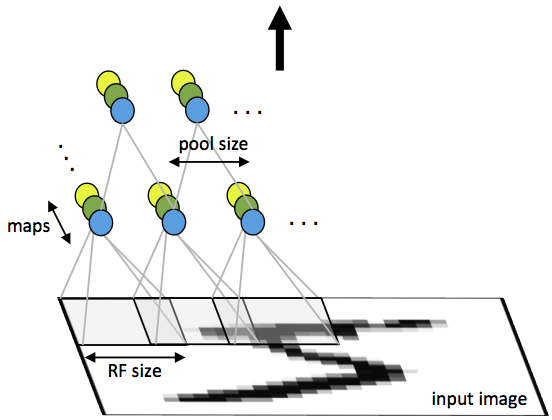
\includegraphics[width=2.60417in,height=\textheight]{Cnn_layer_standford.png}
\caption{Architecture of a convolutive neural network (Stanford credit)}
\end{figure}

\end{frame}

\begin{frame}{Convolution layer}
\protect\hypertarget{convolution-layer}{}

\begin{itemize}
\item
  Image \(\mathcal{I}(u,v,c)\) : each pixelwith \((u,v)\) is described
  by \(C\) color levels (channels), par exemple RGB (red, green, blue)
  \(\Rightarrow\) : array of size (\(M,N,C\))
\item
  Each neuron relies on a linear combination of the signals of a small
  region of the image:
  \[K_{u,v}*\mathcal{I}(c) =  \sum_{n=-k}^{k}\sum_{m=-k}^k K_l(n,m,c)\mathcal{I}\left(u+m,v+n,c \right)\]
\end{itemize}

\[h_{u,v} = \phi(K_{u,v}*\mathcal{I}(c)+b_{u,v})\]

\begin{itemize}
\tightlist
\item
  We obtain a new neuron by moving this window - The amount by which the
  filter shifts is the \textbf{stride} - if we don't move a lot :
  redundancy of information - if we move a lot: loss of information
\end{itemize}

\end{frame}

\begin{frame}{Pooling layer (subsampling)}
\protect\hypertarget{pooling-layer-subsampling}{}

\begin{itemize}
\tightlist
\item
  Averaging or computing maximum on small areas
\item
  \(\phi\) can be applied before or after pooling
\item
  Allows to reduce the dimension (number of variables to be treated) but
  also to make the network less sensitive to possible translations of
  the image
\end{itemize}

\end{frame}

\begin{frame}{Finally}
\protect\hypertarget{finally}{}

\begin{itemize}
\tightlist
\item
  After several layers and convolution / pooling, we apply one or more
  layers of \emph{fully connected layers} (= network shown before)
\end{itemize}

\end{frame}

\begin{frame}{Towards increasingly complex network architectures}
\protect\hypertarget{towards-increasingly-complex-network-architectures}{}

\begin{itemize}
\item
  Networks now much more complex
\item
  Can be processed with Graphical Processor Unit (GPU) cards
\item
  Results of the \emph{Large Scale Visual Recognition Challenge
  (ILSVRC)}
\end{itemize}

\begin{figure}
\centering
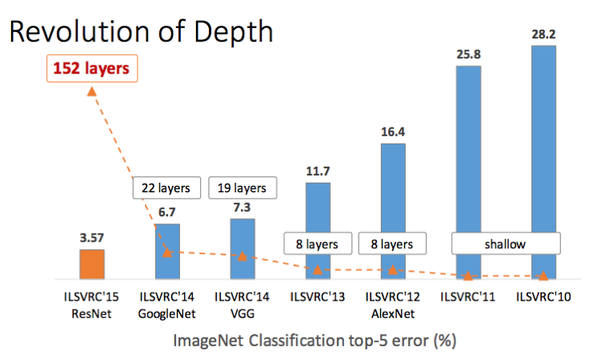
\includegraphics[width=2.60417in,height=\textheight]{depth_error.png}
\caption{Error rate and depths of the network}
\end{figure}

\end{frame}

\hypertarget{conclusion}{%
\section{Conclusion}\label{conclusion}}

\begin{frame}[fragile]{Conclusion}
\protect\hypertarget{conclusion-1}{}

\begin{itemize}
\item
  Ultra-fast vision of the definition of a deep neural network
\item
  In practice: expertise is based on how to combine layers and different
  types of neurons (see practice here after)
\item
  References: - Wikipedia - Wikistat course by Philippe Besse (Toulouse)
  - Reference book: Deep Learning by Yoshua Bengio
  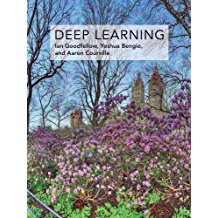
\includegraphics[width=0.52083in,height=\textheight]{livre_bengio.jpg}

\begin{verbatim}
- Video https://www.college-de-france.fr/site/yann-lecun/course-2016-02-12-14h30.htm
- Results and conferences by Francis Bach
\end{verbatim}
\end{itemize}

\end{frame}

\end{document}
